\documentclass{report}
% package para el simbolo dotminus
\usepackage{amsmath}

% macro para dotminus
\makeatletter
\newcommand{\dotminus}{\mathbin{\text{\@dotminus}}}
\newcommand{\@dotminus}{%
  \ooalign{\hidewidth\raise1ex\hbox{.}\hidewidth\cr$\m@th-$\cr}%
}
\makeatother


\input{preamble}
\input{macros}
\input{letterfonts}

\title{\Huge{Some Class}\\Random Examples}
\author{\huge{Your Name}}
\date{}

\begin{document}

\maketitle
\newpage% or \cleardoublepage
% \pdfbookmark[<level>]{<title>}{<dest>}
\pdfbookmark[section]{\contentsname}{toc}
\tableofcontents
\pagebreak

\chapter{}

\qs{}{
	$\textbf{Ejercicio 1. }$  Mostrar que,  dado un k fijo, la función constante $f(x)=k$ puede defnirse usando
	las funciones iniciales y composición $(sin$ usar recursión primitiva).
}
\sol Cualquier $ k \in \mathbb{N}$ puede ser construido aplicando sucesivamente la funcion $s(x)$ a la funcion $n(x)$.
\begin{align}
	f(x)= s_k (x) = \underbrace{s(s(\ldots s(n(x))\ldots))}_{k\ \text{veces}}
\end{align}

Ya que $s(n(x))$ es composicion de funciones primitivas, es primitiva recursiva.
Razonando de forma inductiva, cada vez que aplicamos $s(x)$ a un cierto $s_{k-1} (x)$, obtenemos un $s_k (x)$ que de nuevo, por composicion, es primitiva recursiva.




\qs{}{

	Ejercicio 2. Probar que las signicntes funciones son primitivas recursivas, mostrando que pueden
	obtenerse a partir des funciones iniciales usando composición y/o recursion primitiva:

	$\begin{aligned}
		\\
		&f_1(x,y)=x+y\quad f_2(x,y)=x\cdot y\quad f_3(x,y)=x^y\quad f_4(x,y)=\underbrace{x^{x^{x^{\cdot^{\cdot^{\cdot^{\cdot^{x}}}}}}}}_{y\ \text{veces}}\\
		\\
		&g_1(x)=x \dotminus 1\quad g_2(x,y)=x \dotminus y\quad g_3(x,y)=\max\{x,y\}\quad g_4(x,y)=\min\{x,y\}\\
		\\
		&Observaciones:\text{Se asume que }f_4(x,0)=1.\quad x\dotminus y=\begin{cases}x-y&\text{si }y\leq x\\
			0&\text{si }y>x\end{cases}
	\end{aligned}$
}

\sol $f_1(x,y) = x+y$
\begin{align*}
	f_1(x,0) &= 0 = n(x)\\
	f_1(x,y) &= \underbrace{((\ldots((0+1)+1)\ldots+1)+1)+1}_{y \ veces}\\
	f_1(x,y) &= f_1(x,y-1)+1\\
			 &= s(f_1(x,y-1))\\
\end{align*}

Pero para que cierre la aridad con el esquema de recursion primitiva, debemos encontrar una funcion g tal que:
$f_1(x,y) = g(f(x,y-1),x,y-1)$, esto se arregla tomando $g(x,y,z) = s(u_1^3(x,y,z))$
Entonces nos queda:
\begin{align}
	f_1(x,y) = g(f(x,y-1),x,y-1) = s(u_1^3(f(x,y-1),x,y-1))
\end{align}

\sol $f_{2}(x,y)=x.y$
\begin{align*}
	&f_{2}(x,0)=n(x) \\
	&f_2(x,y)=f_2(x,y-1)+x=f_1(f_2(x,y-1),x)\\
	&f_{2}(x,y)= f1(u_1^3(f_2(x,y-1),x,y-1),\ u_2^3(f_2(x,y-1),x,y-1))\\
	&f_{2}(x,y)= g(f_2(x,y-1),x,y-1)
\end{align*}

Con $g(x,y,z) = f_1(u_1^3(x,y,z),u_2^3(x,y,z))$, ya que $g$ se obtiene por coposicion de funciones PR, entonces tambien es PR.

~

\sol $f_{3}(x,y)=x^{y}$
\begin{align*}
	&f_{3}(x,0)=1\\
	&f_{3}(x,y)=f_{3}(x,y-1).x=f_{2}(f_{3}(x,y-1),x)\\
	&f_{3}(x,y)=f_{2}(u_{1}^{3}(f_{3}(x,y-1),x,y-1),u_{2}^{3}(f_{3}(x,y-1),x,y-1))\\
	&f_{3}(x,y)= g(f_3(x,y-1),x,y-1)
\end{align*}

Con $g(x,y,z) = f_2(u_1^3(x,y,z),u_2^3(x,y,z))$, ya que $g$ se obtiene por coposicion de funciones PR, entonces tambien es PR.

~

\sol 
$f_4(x,y)=\underbrace{x^{x^{x^{\cdot^{\cdot^{\cdot^{\cdot^{x}}}}}}}}_{y\ \text{veces}}$
\begin{align*}
	&f_{4}(x,0)=1\\
	&f_{4}(x,y)=f_{4}(x,y-1)^{x}=f_{3}(f_{4}(x,y-1),x)\\
	&f_{4}(x,y)=f_{3}(u_{1}^{3}(f_{4}(x,y-1),x,y-1),u_{2}^{3}(f_{4}(x,y-1),x,y-1))
\end{align*}

Con $g(x,y,z) = f_3(u_1^3(x,y,z),u_2^3(x,y,z))$, ya que $g$ se obtiene por coposicion de funciones PR, entonces tambien es PR.

~

\sol
$g_1(x)=x \dotminus 1$
\begin{align*}
	&g_{1}(0)=n(x)\\&g_{1}(x)=u_{2}^{2}(g_{1}(x),x-1)
\end{align*}

~

\sol
$g_2(x,y)=x \dotminus y$
\begin{align*}
	&g_{2}(x,0)=u_{1}^{1}(x)\\
	&g_{2}(x,y)=g_{2}(x,y-1)-1=g_{1}(g_{2}(x,y-1))\\
	&g_{2}(x,y)=g_{1}(u_{1}^{3}(g_{2}(x,y-1),x,y-1))\\
	&g_{2}(x,y)=g(g_{2}(x,y-1),x,y-1)
\end{align*}

Con $g(x,y,z) = g_2(u_1^3(x,y,z))$, ya que $g$ se obtiene por coposicion de funciones PR, entonces tambien es PR.

~

\sol
$g_3(x,y)=\max\{x,y\}$
\begin{align*}
	&\max\{x,y\}=(x\leqslant y).y+\alpha(x\leqslant y).x\\
	&\max\{x,y\}=f_{2}((x\leqslant y),y)+f_{2}(\alpha(x\leqslant y),y)\\
	&\max\{x,y\}=f_{1}(\underbrace{f_{2}((x\leqslant y),y)}_{h_{1}},\underbrace{f_{2}(\alpha(x\leqslant y),y)}_{h_{2}})
\end{align*}

Las funciones $\alpha$ (negacion) y $\leq$ son las definidas en la clase teorica numero 2.
Se puede probar por composicion que $h_1$ y $h_2$ son PR. Por lo tanto queda demostrado por composicion que $g_3$ tambien es PR.

~

\sol
$g_4(x,y)=\min\{x,y\}$
\begin{align*}
	&\min\{x,y\}=(x\leqslant y).x+\alpha(x\leqslant y).y\\
	&\min\{x,y\}=f_{2}((x\leqslant y).x)+f_{2}(\alpha(x\leqslant y),y)\\
	&\min\{x,y\}=f_{1}(\underbrace{f_{2}((x\leqslant y),y)}_{h_{1}},\underbrace{f_{2}(\alpha(x\leqslant y),y)}_{h_{2}})
\end{align*}

Las funciones $\alpha$ (negacion) y $\leq$ son las definidas en la clase teorica numero 2.
Se puede probar por composicion que $h_1$ y $h_2$ son PR. Por lo tanto queda demostrado por composicion que $g_3$ tambien es PR.






\qs{}{
	Ejercicio 3. Sea $\mathcal{C}_i$ la clase de funciones iniciales, es decir, aquella que contiene a:\\\\
	$n( x) = 0$ \ \ \ \ $s( x) = x+ 1$ \ \ \ \ 
	$u_i^n(x_1,\ldots,x_n)=x_i$ para cada $n\in\mathbb{N}$ e $i\in\{1,\ldots,n\}$\\

	$\begin{aligned}&\text{y sea }\mathcal{C}_c\text{ la (mínima) clase que extiende a }\mathcal{C}_i\text{ y se encuentra cerrada por composición, i.e., si}\\&f,g_1,\ldots g_m\text{ están en }\mathcal{C}_c,\text{ entonces }h(x_1,\ldots,x_n)=f(g_1(x_1,\ldots,x_n),\ldots,g_m(x_1,\ldots,x_n))\text{ también}\\&\text{lo está.}\end{aligned}$
	\\\\a. Demostrar que para toda $f: \mathbb{N} ^n\to \mathbb{N} , f\text{ est\' {a} en }\mathcal{C} _c$ sii existe $k\geq0$ tal que, o bien sucede
	$f(x_1,\ldots,x_n)=k$, o bien para algún $i$ fijo, se tiene $f(x_1,\ldots,x_n)=x_i+k.$
	\\\\b. Mostrar que existe una función primitiva recursiva que no está en $\mathcal{C}_c.$
}

\sol a)

($\rightarrow$)

Vamos a usar induccion estructural

Casos Base:
Veamos que se cumple para las funciones iniciales
\begin{align*}
	&n(x)=0,\ \ k=0\\
	&s(x)=x+1,\ \ k=1\\
	&u_i^n(x_1,...,x_n)=x_i+0,\ \ k=0
\end{align*}
\\
Paso inductivo:\\
Sea $f \in \mathcal{C}$, $f(x_1, \ldots, x_n) = h(g_1(x1, \ldots, x_n), \ldots, g_n(x1, \ldots, x_n))$.
Veamos que o bien $f(x_1, \ldots, x_n) = k$, o bien  $f(x_1, \ldots, x_n) = x_i + k$
\\\\
Las funciones que componen a h, cumplen con la HI. Por lo tanto, separemos en casos:
\\\\
Caso $h(x1, \ldots, x_n) = k$: Entonces tenemos que $f(x1, \ldots, x_n) = k = k'$, ya esta!
\\\\
Caso $h(x1, \ldots, x_n) = x_i + k'$: Entonces tenemos que $f(x1, \ldots, x_n) = g_i(x1, \ldots, x_n)$.

Ahora tenemos 2 sub-casos mas:

Caso $g_i(x1, \ldots, x_n) = k''$:  $f(x1, \ldots, x_n) = k' + k'' = k$

Caso $g_i(x1, \ldots, x_n) = x_j + k''$: $f(x1, \ldots, x_n) = x_j + k'' + k' = x_j + k$
\\
En ambos casos, vemos que se cumple lo que queriamos.
\\\\

($\leftarrow$)\\
Ya vimos que la funcion $h_k(x) = k$, puede ser definida por composicion y recursion a partir de
las funciones iniciales, entonces $h_k \in \mathcal{C}$.
Entonces $f(x_1 , \ldots , x_n) = h_k(u_1^n(x_1 , \ldots , x_n)) = k$, xlt $f \in \mathcal{C}$
\\\\
Se puede defnir la funcion $s_k(x) = x + k$ usando sucesivamente la funcion $s$, por composicion $s_k \in \mathcal{C}$.
Xlt $f(x_1, ... , x_n) = x_i  + k = s_k(u_i^n(x_1, ... , x_n))$. Y esta ultima al ser composicion de funciones de
$\mathcal{C}$, nos asegura que f tambien esta en $\mathcal{C}$.





\qs{}{}
\qs{}{}
\qs{}{}
\qs{}{}
\qs{}{}
\qs{}{}
\qs{}{}





\section{Random Examples}
\dfn{Limit of Sequence in $\bs{\bbR}$}{Let $\{s_n\}$ be a sequence in $\bbR$. We say $$\lim_{n\to\infty}s_n=s$$ where $s\in\bbR$ if $\forall$ real numbers $\eps>0$ $\exists$ natural number $N$ such that for $n>N$ $$s-\eps<s_n<s+\eps\text{ i.e. }|s-s_n|<\eps$$}
\qs{}{Is the set ${x-}$axis${\setminus\{\text{Origin}\}}$ a closed set}
\sol We have to take its complement and check whether that set is a open set i.e. if it is a union of open balls
\nt{We will do topology in Normed Linear Space  (Mainly $\bbR^n$ and occasionally $\bbC^n$)using the language of Metric Space}
\clm{Topology}{}{Topology is cool}
\ex{Open Set and Close Set}{
	\begin{tabular}{rl}
		Open Set:   & $\bullet$ $\phi$                                              \\
		            & $\bullet$ $\bigcup\limits_{x\in X}B_r(x)$ (Any $r>0$ will do) \\[3mm]
		            & $\bullet$ $B_r(x)$ is open                                    \\
		Closed Set: & $\bullet$ $X,\ \phi$                                          \\
		            & $\bullet$ $\overline{B_r(x)}$                                 \\
		            & $x-$axis $\cup$ $y-$axis
	\end{tabular}}
\thm{}{If $x\in$ open set $V$ then $\exists$ $\delta>0$ such that $B_{\delta}(x)\subset V$}
\begin{myproof}By openness of $V$, $x\in B_r(u)\subset V$
	\begin{center}
		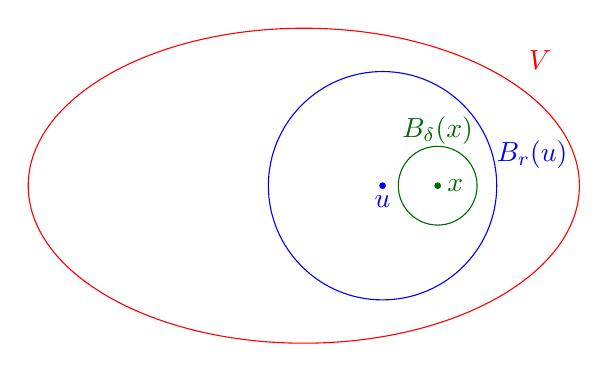
\begin{tikzpicture}
			\draw[red] (0,0) circle [x radius=3.5cm, y radius=2cm] ;
			\draw (3,1.6) node[red]{$V$};
			\draw [blue] (1,0) circle (1.45cm) ;
			\filldraw[blue] (1,0) circle (1pt) node[anchor=north]{$u$};
			\draw (2.9,0.4) node[blue]{$B_r(u)$};
			\draw [green!40!black] (1.7,0) circle (0.5cm) node [yshift=0.7cm]{$B_{\delta}(x)$} ;
			\filldraw[green!40!black] (1.7,0) circle (1pt) node[anchor=west]{$x$};
		\end{tikzpicture}
	\end{center}

	Given $x\in B_r(u)\subset V$, we want $\delta>0$ such that $x\in B_{\delta} (x)\subset B_r(u)\subset V$. Let $d=d(u,x)$. Choose $\delta $ such that $d+\delta<r$ (e.g. $\delta<\frac{r-d}{2}$)

	If $y\in B_{\delta}(x)$ we will be done by showing that $d(u,y)<r$ but $$d(u,y)\leq d(u,x)+d(x,y)<d+\delta<r$$
\end{myproof}

\cor{}{By the result of the proof, we can then show...}
\mlenma{}{Suppose $\vec{v_1}, \dots, \vec{v_n} \in \RR[n]$ is subspace of $\RR^n$.}
\mprop{}{$1 + 1 = 2$.}

\section{Random}
\dfn{Normed Linear Space and Norm $\boldsymbol{\|\cdot\|}$}{Let $V$ be a vector space over $\bbR$ (or $\bbC$). A norm on $V$ is function $\|\cdot\|\ V\to \bbR_{\geq 0}$ satisfying \begin{enumerate}[label=\bfseries\tiny\protect\circled{\small\arabic*}]
		\item \label{n:1}$\|x\|=0 \iff x=0$ $\forall$ $x\in V$
		\item \label{n:2}	$\|\lambda x\|=|\lambda|\|x\|$ $\forall$ $\lambda\in\bbR$(or $\bbC$), $x\in V$
		\item \label{n:3} $\|x+y\| \leq \|x\|+\|y\|$ $\forall$ $x,y\in V$ (Triangle Inequality/Subadditivity)
	\end{enumerate}And $V$ is called a normed linear space.

	$\bullet $ Same definition works with $V$ a vector space over $\bbC$ (again $\|\cdot\|\to\bbR_{\geq 0}$) where \ref{n:2} becomes $\|\lambda x\|=|\lambda|\|x\|$ $\forall$ $\lambda\in\bbC$, $x\in V$, where for $\lambda=a+ib$, $|\lambda|=\sqrt{a^2+b^2}$ }


\ex{$\bs{p-}$Norm}{\label{pnorm}$V={\bbR}^m$, $p\in\bbR_{\geq 0}$. Define for $x=(x_1,x_2,\cdots,x_m)\in\bbR^m$ $$\|x\|_p=\Big(|x_1|^p+|x_2|^p+\cdots+|x_m|^p\Big)^{\frac1p}$$(In school $p=2$)}
\textbf{Special Case $\bs{p=1}$}: $\|x\|_1=|x_1|+|x_2|+\cdots+|x_m|$ is clearly a norm by usual triangle inequality. \par
\textbf{Special Case $\bs{p\to\infty\ (\bbR^m$ with $\|\cdot\|_{\infty})}$}: $\|x\|_{\infty}=\max\{|x_1|,|x_2|,\cdots,|x_m|\}$\\
For $m=1$ these $p-$norms are nothing but $|x|$.
Now exercise
\qs{}{\label{exs1}Prove that triangle inequality is true if $p\geq 1$ for $p-$norms. (What goes wrong for $p<1$ ?)}
\sol{\textbf{For Property \ref{n:3} for norm-2}	\subsubsection*{\textbf{When field is $\bbR:$}} We have to show\begin{align*}
		         & \sum_i(x_i+y_i)^2\leq \left(\sqrt{\sum_ix_i^2} +\sqrt{\sum_iy_i^2}\right)^2                                       \\
		\implies & \sum_i (x_i^2+2x_iy_i+y_i^2)\leq \sum_ix_i^2+2\sqrt{\left[\sum_ix_i^2\right]\left[\sum_iy_i^2\right]}+\sum_iy_i^2 \\
		\implies & \left[\sum_ix_iy_i\right]^2\leq \left[\sum_ix_i^2\right]\left[\sum_iy_i^2\right]
	\end{align*}So in other words prove $\langle x,y\rangle^2 \leq \langle x,x\rangle\langle y,y\rangle$ where
	$$\langle x,y\rangle =\sum\limits_i x_iy_i$$

	\begin{note}
		\begin{itemize}
			\item $\|x\|^2=\langle x,x\rangle$
			\item $\langle x,y\rangle=\langle y,x\rangle$
			\item $\langle \cdot,\cdot\rangle$ is $\bbR-$linear in each slot i.e. \begin{align*}
				      \langle rx+x',y\rangle=r\langle x,y\rangle+\langle x',y\rangle	\text{ and similarly for second slot}
			      \end{align*}Here in $\langle x,y\rangle$ $x$ is in first slot and $y$ is in second slot.
		\end{itemize}
	\end{note}Now the statement is just the Cauchy-Schwartz Inequality. For proof $$\langle x,y\rangle^2\leq \langle x,x\rangle\langle y,y\rangle $$ expand everything of $\langle x-\lambda y,x-\lambda y\rangle$ which is going to give a quadratic equation in variable $\lambda $ \begin{align*}
		\langle x-\lambda y,x-\lambda y\rangle & =\langle x,x-\lambda y\rangle-\lambda\langle y,x-\lambda y\rangle                                       \\
		                                       & =\langle x ,x\rangle -\lambda\langle x,y\rangle -\lambda\langle y,x\rangle +\lambda^2\langle y,y\rangle \\
		                                       & =\langle x,x\rangle -2\lambda\langle x,y\rangle+\lambda^2\langle y,y\rangle
	\end{align*}Now unless $x=\lambda y$ we have $\langle x-\lambda y,x-\lambda y\rangle>0$ Hence the quadratic equation has no root therefore the discriminant is greater than zero.

	\subsubsection*{\textbf{When field is $\bbC:$}}Modify the definition by $$\langle x,y\rangle=\sum_i\overline{x_i}y_i$$Then we still have $\langle x,x\rangle\geq 0$}

\section{Algorithms}
\begin{algorithm}[H]
	\KwIn{This is some input}
	\KwOut{This is some output}
	\SetAlgoLined
	\SetNoFillComment
	\tcc{This is a comment}
	\vspace{3mm}
	some code here\;
	$x \leftarrow 0$\;
	$y \leftarrow 0$\;
	\uIf{$ x > 5$} {
		x is greater than 5 \tcp*{This is also a comment}
	}
	\Else {
		x is less than or equal to 5\;
	}
	\ForEach{y in 0..5} {
		$y \leftarrow y + 1$\;
	}
	\For{$y$ in $0..5$} {
		$y \leftarrow y - 1$\;
	}
	\While{$x > 5$} {
		$x \leftarrow x - 1$\;
	}
	\Return Return something here\;
	\caption{what}
\end{algorithm}

\end{document}
